\clearpage
\section{Autonomous Vehicles and Robots}

Autonomous robots or vehicles can work for an extended period of time gathering information from its surroundings to be able to work without human intervention. The robot or vehicles gathers different kinds of data, depending on what the goal of the robot it.Positional data can be utilized for navigation and path finding in a known and unknown environment. Intelligent autonomous devices are able to adapt to changes happening in its surroundings.
Currently there are many robots on the market that are self-reliant, ranging from autonomous vacuum cleaner to drones and helicopters. \cite{autonomousbasic}

Simple autonomous robots use ultrasonic sensors or infrared to manipulate itself if it detects obstacles. The is useful for obstacle avoidance and mapping of unknown areas, where the robot through a reference point can pin-point the obstacles it has encountered along the way.
More advanced robots use vision to grant them the ability to see their surroundings, algorithms analyse the camera data and gives the robot depth perception, which grants the robot the ability to instantly identify objects and locate them immediately.\cite{obstacles}

There exists two kinds of autonomous robots, a single computer autonomous robot and insect robots. The single computer autonomous robot uses its own on-board computing unit to do its computations and decisions, whereas the the insect robots are a fleet a many robots who are controlled by a single separate computing unit.
The advantage of having a single computer autonomous robot is that the tasks it performs can be done using more computer resources. It has the possibility of utilizing the computing power to its full potential, instead of relying on a separate unit that is also making decisions and calculations for many other robots.
The individual robot in the insect family is simple, but the whole robot fleet can be advanced and possibly perform sophisticated tasks, that a require multiple simpler robots.\cite{singleandinsect}


\clearpage
\section{Path finding and mapping}

Pathfinding is done by a computer, where it uses plotting to find the shortest path between two different points. It can be viewed as a more efficient way of navigating a maze. The main objective is getting from some location to a goal location.
There exists pathfinding algorithms that are used for software simulations, but also for mobile robot navigation. A common pathfinding algorithm is A* (pronounced A star) and its extended version named D* (Dynamic A*).

\begin{figure}[H]
\centering
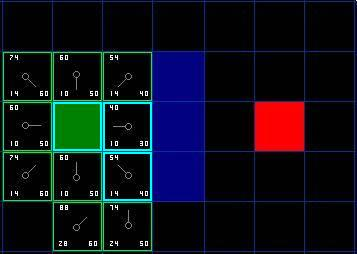
\includegraphics[width=.7\linewidth]{images/aStar2.jpg}
\caption{Upper-left number is F, Lower-left G and Lower-right H}
\label{fig:sub2}
\end{figure}

The A* algorithm is most commonly used in video games. The algorithm determines that cost of movement from the start to the given generated destination(G), in relation to the estimated cost of movement to its final destination(H). Based on the current destination the possible surrounding paths are analysed and the path with the F value(F = G + H)becomes the chosen path.\cite{astar}

In the early stages of robot automation, it was assumed that the environment around the robot was known and the path was generated based on this. This was okay until the robot started to meet inconsistencies and obstacles in the path (This being discrepancies between the true state and the world state), the robot then either had to re-plan completely from scratch or alter the plan through trial-and-error. Computational wise, it would require too much power to re-plan from scratch (Even though this is the optimal choice) and most of the time trial-and-error does not yield an optimal outcome.


\clearpage
\begin{figure}[H]
        \centering
        \begin{subfigure}[H]{0.4\textwidth}
                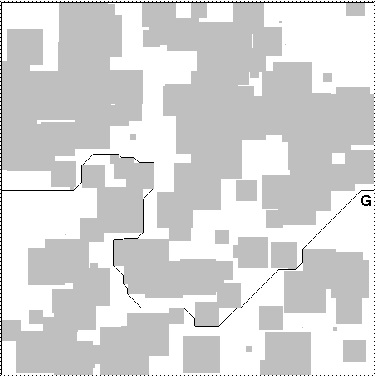
\includegraphics[width=\textwidth]{images/completemap.jpg}
                \caption{Complete Map}
                \label{fig:completemap}
        \end{subfigure}%
\quad
        \begin{subfigure}[H]{0.4\textwidth}
                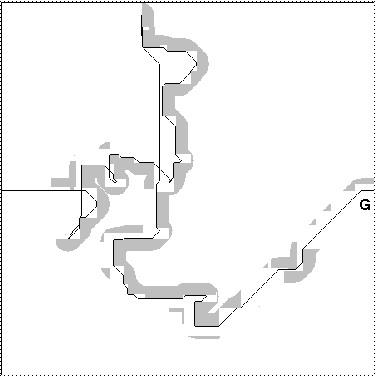
\includegraphics[width=\textwidth]{images/optimisticmap.jpg}
                \caption{Optimistic Map}
                \label{fig:optimisticmap}
        \end{subfigure}
        \caption{Mapping simulations with D*\cite{dstar}}\label{fig:animals}
\end{figure}

The D* algorithm creates an initial path based on assumed and known information, it then edits the path based on new information it receives whilst navigating the path. The final version of the edited plan is equivalent to replanning the whole thing from scratch, but avoids the limitations of the computation power.
Whenever an on-board sensor receives information about an obstacle, the algorithm can edit the path based on what possible routes there are available near by.
D* is fast at navigating large scale unknown environments because during its exploration its able to edit and repair its desired path and navigate towards its goal. It would require too much effort to re-plan everything from scratch every time it failed, especially for large scale environments.\cite{dstar}\cite{moredstar}

The figure(a) shows the map where the given robot knowns it's environment (The grey boxes) and can therefore easily determine the optimal path or the "Complete Map" in this case. Figure (b) on the other hand shows the "Optimistic Map", since before navigating on the planned path it assumes that there are no obstacles. Whenever the robot meets an obstacle during the optimistic map, it adjust it's course to continue towards its goal. On figure (b) it only displays the obstacles which it met during its navigation along the path.




\clearpage
Simple autonomous robots navigate by the use of infrared LEDs or by the use of photo-resistors and LEDS, by following lines drawn on a surface.\\
%http://www.ikalogic.com/line-tracking-sensors-and-algorithms/ <-- for the line tracking 
Some autonomous robots and vehicles use multiples of different range sensors and other sensory equipment, to map and locate themselves in indoor and outdoor environments. The map that is generated can be used to keep track of static items in the environment such as structures and difference in terrain, but the map also distinguishes non-static items such as humans and other moving objects. Since the maps are created by the vehicle itself whilst exploring, this technology can be used with or without GPS\cite{rangesens}\cite{rangesensarc}.  Robots and vehicles have been created using this technology to explore known and unknown environments. Because of advanced algorithms and hardware these autonomous devices are capable of performing tasks more efficiently than humans, but also in places that are unsafe and hard to reach.

Autonomous robots also use these tools to work together. Using a shared map, the robots can keep track of one another and either perform tasks together or separately, depending on what is required from them.

\begin{figure}[H]
	\centering
	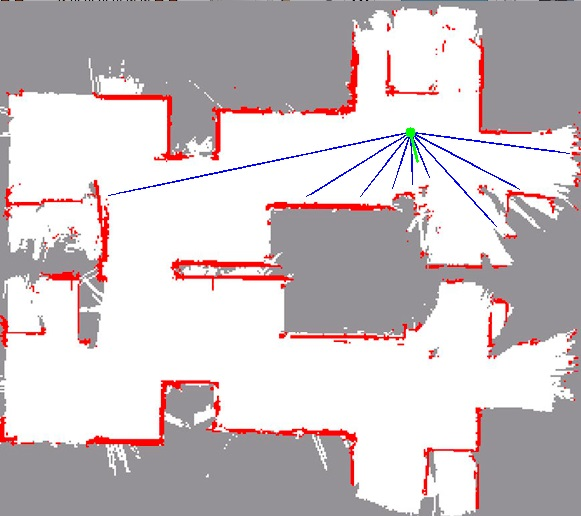
\includegraphics[scale=.7]{images/laserrangemap.jpg}
	\caption{Laser Range Map\cite{laserrangepic}}
	\label{fig:laserrangemap}
\end{figure}

Laser range finders and sonar arrays are used to navigate and determine the shortest possible path to a given destination. The sensory equipment is used to give the autonomous robot a sense of distance towards objects in an environment, giving it vital data regarding optimal travel directions\cite{lasersonar}.


%http://www.kuka-labs.com/en/service_robotics/mobile_robotics/autonomous_navigation/

%Advanced imagery stufferino
%http://ilab.usc.edu/publications/doc/Siagian_etal13icra.pdf

%Misc
%http://www.doc.ic.ac.uk/~nd/surprise_97/journal/vol4/jmd/
%http://www.doc.ic.ac.uk/~nd/surprise_97/journal/vol1/jmd/


